% This must be in the first 5 lines to tell arXiv to use pdfLaTeX, which is strongly recommended.
\pdfoutput=1
% In particular, the hyperref package requires pdfLaTeX in order to break URLs across lines.

\documentclass[11pt]{article}

% Change "review" to "final" to generate the final (sometimes called camera-ready) version.
% Change to "preprint" to generate a non-anonymous version with page numbers.
% \usepackage[final]{acl}
\usepackage[review]{acl}

% Standard package includes
\usepackage{times}
\usepackage{latexsym}
\usepackage{graphicx}
\usepackage{amsmath}
\usepackage{amsfonts}
% For proper rendering and hyphenation of words containing Latin characters (including in bib files)
\usepackage[T1]{fontenc}
% For Vietnamese characters
% \usepackage[T5]{fontenc}
% See https://www.latex-project.org/help/documentation/encguide.pdf for other character sets



% This assumes your files are encoded as UTF8
\usepackage[utf8]{inputenc}
\usepackage{CJKutf8}
\usepackage{subcaption}
\usepackage{hyperref}

% This is not strictly necessary, and may be commented out,
% but it will improve the layout of the manuscript,
% and will typically save some space.
\usepackage{microtype}
\usepackage{lscape}

% This is also not strictly necessary, and may be commented out.
% However, it will improve the aesthetics of text in
% the typewriter font.
\usepackage{inconsolata}
\usepackage{xcolor}
\usepackage{tipa}
\usepackage{multirow}
\usepackage{array}


\newcommand{\MY}[1]{\textcolor{blue}{(Mengyue: #1)}}
\newcommand{\KZ}[1]{\textcolor{red}{(Kenny: #1)}}
\newcommand{\HA}[1]{\textcolor{brown}{(Haoan: #1)}}
\newcommand{\YV}[1]{\textcolor{magenta}{(Yvonne: #1)}}
\newcommand{\XJ}[1]{\textcolor{orange}{(Xiujie: #1)}}
\newcommand{\secref}[1]{Sec. \ref{#1}}
\newcommand{\figref}[1]{Figure \ref{#1}}
\newcommand{\eqnref}[1]{Eq. (\ref{#1})}
\newcommand{\tabref}[1]{Table \ref{#1}}
\newcommand{\exref}[1]{Example \ref{#1}}
\newcommand{\appref}[1]{Appendix \ref{#1}}

% If the title and author information does not fit in the area allocated, uncomment the following
%
%\setlength\titlebox{<dim>}
%
% and set <dim> to something 5cm or larger.

\title{Automatic Reconstruction of Ancient Chinese Pronunciations}

% Author information can be set in various styles:
% For several authors from the same institution:
% \author{Author 1 \and ... \and Author n \\
%         Address line \\ ... \\ Address line}
% if the names do not fit well on one line use
%         Author 1 \\ {\bf Author 2} \\ ... \\ {\bf Author n} \\
% For authors from different institutions:
% \author{Author 1 \\ Address line \\  ... \\ Address line
%         \And  ... \And
%         Author n \\ Address line \\ ... \\ Address line}
% To start a separate ``row'' of authors use \AND, as in
% \author{Author 1 \\ Address line \\  ... \\ Address line
%         \AND
%         Author 2 \\ Address line \\ ... \\ Address line \And
%         Author 3 \\ Address line \\ ... \\ Address line}

\author{First Author \\
  Affiliation / Address line 1 \\
  Affiliation / Address line 2 \\
  Affiliation / Address line 3 \\
  \texttt{email@domain} \\\And
  Second Author \\
  Affiliation / Address line 1 \\
  Affiliation / Address line 2 \\
  Affiliation / Address line 3 \\
  \texttt{email@domain} \\}

\begin{document}
\maketitle
%\begin{abstract}
%  In the age of information explosion, search engines have been an
%  essential tool in people's daily life and query suggestion is one
%  of most useful feature for a standard search engine. However, because
%  most of search engines are keyword-based, many fantastic features would
%  fail when facing concept-based queries, so does query suggestion. In this
%  paper, we propose a framework so that search engines can give acceptable
%  suggestions when facing concept-based queries.
%\end{abstract}

\begin{abstract}
  A class of search queries which contain abstract concepts are studied in
this paper. These queries cannot be correctly interpreted by traditional keyword-based search engines.
  This paper presents a simple framework that detects and instantiates the
abstract concepts by their concrete entities or meanings to produce alternate
queries that yield better search results.
\footnote{Kenny Q. Zhu (corresponding author) is partially
supported by NSFC grants 61100050 and 61033002.}
\end{abstract}

\section{Introduction}
\label{sec:intro}

Evaluation of dialogue systems is an open question. Existing
automatic evaluation metrics for chitchat systems are similar to those for 
other text generation tasks (e.g., machine translation \citep{papineni-etal-2002-bleu}, question-answering \citep{rajpurkar-etal-2016-squad}, 
summarization \citep{lin-2004-rouge}), which depends on calculating word overlaps with 
ground truth reference responses. 
However, for chitchat tasks, there are usually 
many alternative but plausible responses given a situation, 
perhaps more than any other text generation task mentioned above. 
A limited number of reference responses are 
not sufficient to determine how good a generated response is. 
Moreover, such static settings are not good at
assessing an interactive, context-sensitive system.

Interactive human evaluation metrics usually 
involve a Likert scale evaluation after a multi-turn conversation 
with the evaluated bot. 
While this method is a step up from the previous static evaluation, 
it is difficult for human judges to give a concrete score to
any bot.
%\KZ{But are we also asking judges to score invidividual bots, which is difficult?} 
To compare the performance of two bots is easier. 
Thus ACUTE-EVAL~\citep{DBLP:journals/corr/abs-1909-03087} asks the 
judges to make a binary judgment of who is better in conversations between two identical bots 
or between a human and a bot. A more advanced version of that
is \textit{Spot The Bot}~\cite{deriu-etal-2020-spot} which models the 
human evaluation of a 
conversation after the Turing test. Such a process is still 
time-consuming and costly, 
compared with automatic evaluations.

In our opinion, a good method for evaluating multi-turn conversational model/system 
should satisfy the following requirements:
i) be as efficient and inexpensive as possible;
ii) can truly reflect a model's ability to conduct a human conversation; 
iii) evaluation results should correlate well with human judgments;
iv) can be used to compare and rank the capabilities of a set of models/systems.
  
Toward that goal, in this work, we propose an automatic interactive evaluation framework, 
which is called \textit{ChatMatch} for chitchat
agents. This framework can be used to rank any number of bots with very little
time and effort.  Above all, we want to emphasize the significance of
the observation on direct interactions between bots in the evaluation. 
People tend to believe that human-bot conversations are more reliable 
and produce more comprehensive evaluations of chatbots' capabilities. 
This is not always true. As human annotators know their counterpart is a robot, 
they tend to ask common and goal-directed questions. 
The bot-bot chat logs in our experiments show that, surprisingly,  
talking between two different bots may expose both their strengths and weaknesses not seen
in human-bot conversations. 
Here, we take as an example in \figref{fig:two convs} two small fragments 
from the chat logs between humans-bot and bot-bot. While talking about hobbies, 
human keeps asking the bot direct questions, which leads to boring responses from the bot.
However, in a bot-bot setting, two bots, including the same bot in the previous
conversation, start explaining their hobbies to each other, producing a much more natural and 
interesting conversation. 

\begin{figure}[ht!]
\begin{subfigure}{0.5\textwidth}
  \centering
  % include first image
  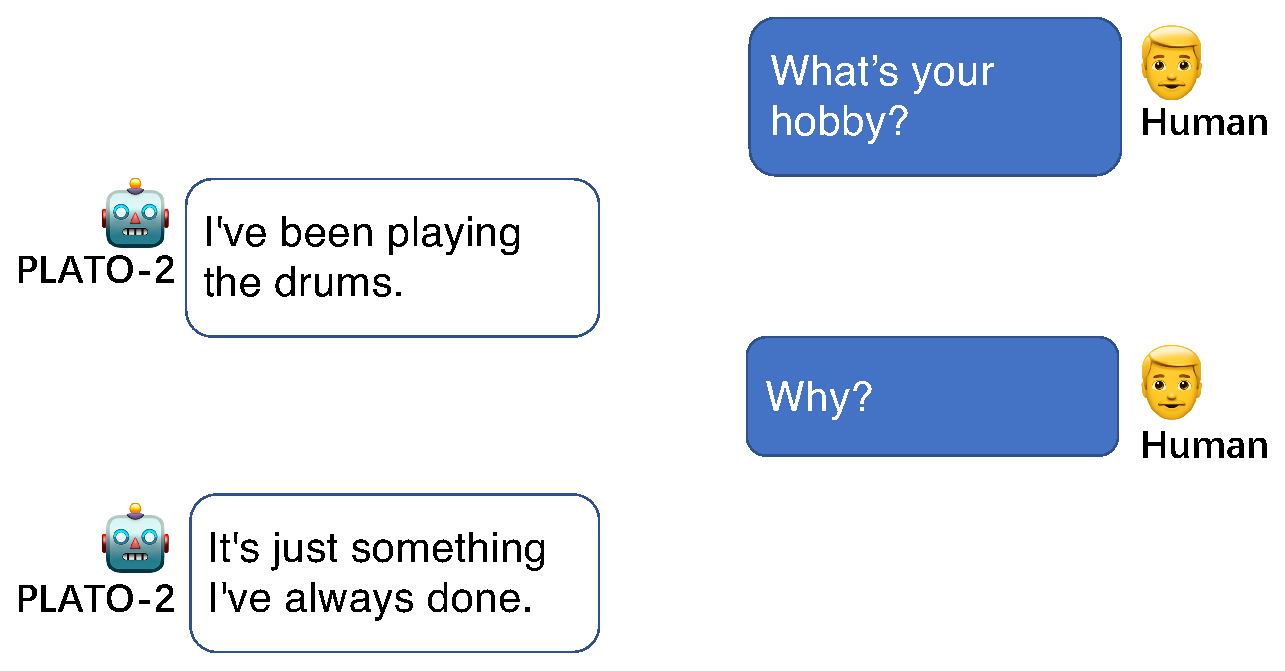
\includegraphics[width=.8\linewidth]{crop1.eps}  
  \caption{A small fragment of conversation between human and bot}
  \label{fig:sub-first}
\end{subfigure}
\begin{subfigure}{0.5\textwidth}
  \centering
  % include second image
  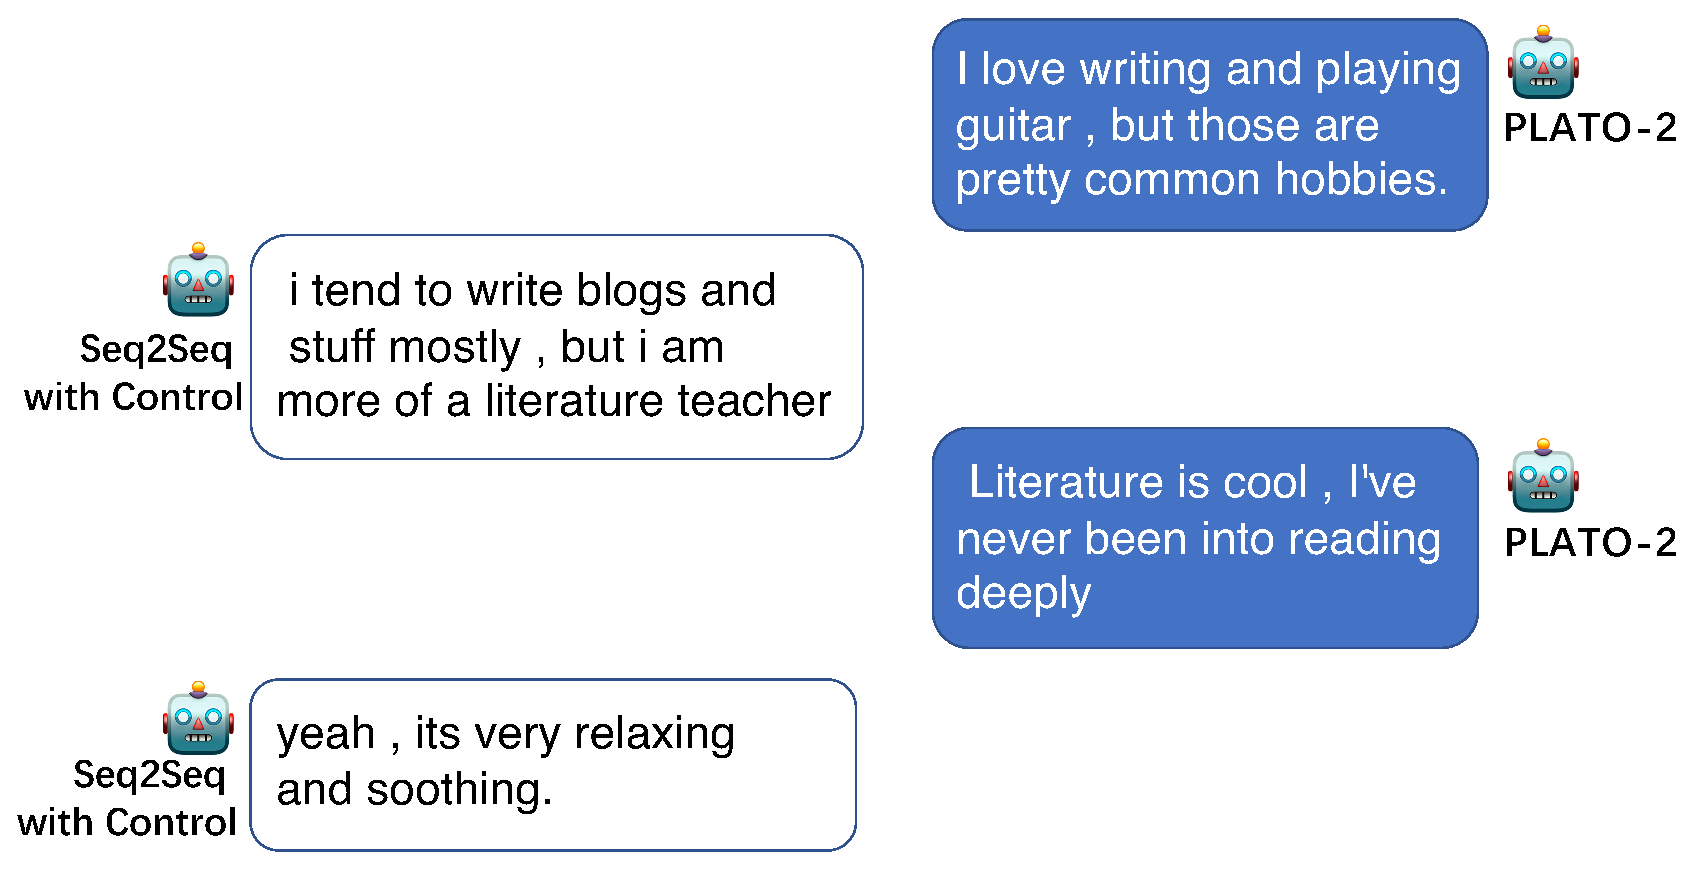
\includegraphics[width=\linewidth]{crop2.eps}  
  \caption{A small fragment of conversation between bot and bot% \KZ{crop the margins
%in this pic or use eps for both.} 
}
  \label{fig:sub-second}
\end{subfigure}
\caption{Small fragments from the chat logs between humans-bot and bot-bot}
\label{fig:two convs}
\end{figure}

Our framework consists of two components: \textit{competition} and 
\textit{scoring}, which may happen simultaneously. The competition is modeled
after most sport tournaments such as soccer or ping pong. 
There are three levels of competitions: 
game-level, match-level and tournament-level. 
Each match consists of several games. During a game, two bots will converse 
freely with each other and a virtual judge will score their performances according to
a group of criteria such as consistency and fluency, etc. 
%As an example like \figref{fig:example} shows, 
%Bot $A$ will be 
%penalized twice for repeating while Bot $B$ will be penalized once for 
%contradicting itself. In addition to the penalty, 
%a bonus point is rewarded to $A$
%who shows to produce relevant response with long term memory. 
%\KZ{Do we still have this as a criterion?}
%However, the specific bonus and penalty settings may vary 
%depending on the domain and scenarios that the experiment is 
%set in. 

%\begin{figure}[th!]
%	\centering
%	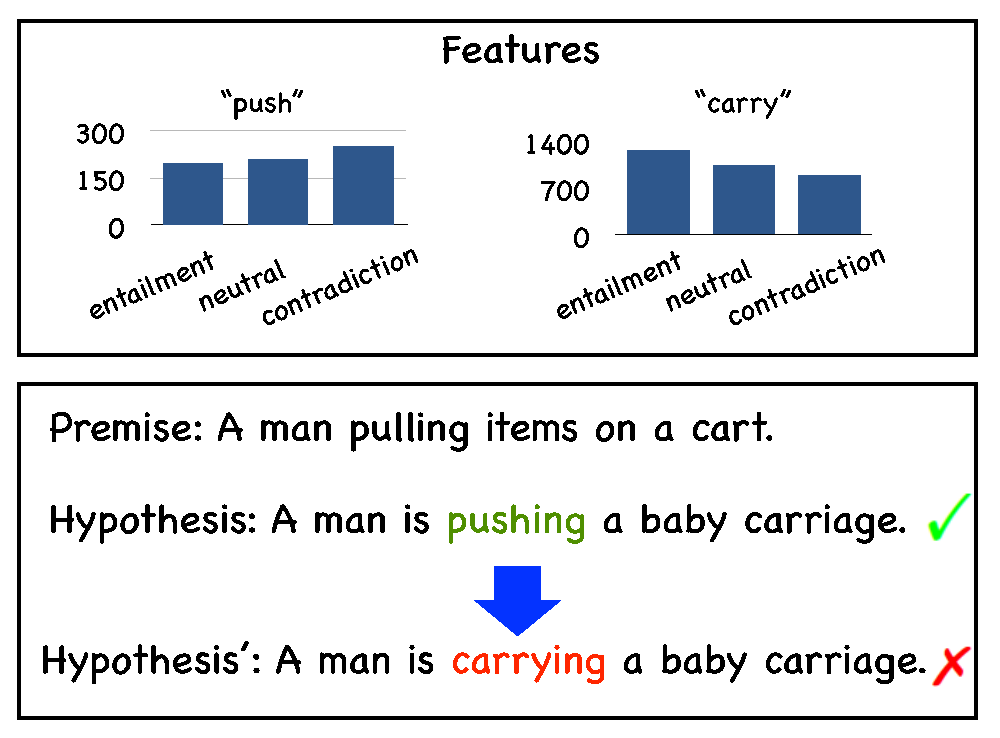
\includegraphics[width=0.95\columnwidth]{example.eps}
%	\caption{A chat snippet between two bots.}
%	\label{fig:example}
%\end{figure}

The main contributions of this paper are:
\begin{itemize}
\item We propose the first interactive evaluation framework for chatbots which
is based solely on bot-to-bot conversations and modeled after sports competitions (\secref{sec:competition}).
\item  The entire scoring process is fully automated and efficient. 
The system can rank seven bots in three minutes on average.
(\secref{sec:scoring}, \secref{sec:time}).
\item  Our experiments show that our scoring system closely tracks the 
human evaluation results. Preliminary results also show
that our evaluation system outperforms 
several recent strong baseline evaluation systems (\secref{sec:main}).
\item %We demonstrate the improvements in efficiency 
%using direct chat logs between bots.
We show that the chats between bots are impressively informative, 
even richer than the chats between humans and bots.
This suggests some possible directions to improve 
the capabilities of bots in the future.
(e.g., by having them learn from each other)  (\secref{sec:diversity})
\end{itemize}

\section{ACP Dataset Construction}\label{sec:dataset}
% When reconstructing the phonetic system, Wang always follows the taxonomy in \textit{Qieyun} and attach pronunciations, represented by phonetic symbols, onto each initial or final category based on \textit{Qieyun} taxonomy. This reconstruction makes use of contemporaneous written materials, primarily poetic and literary materials since these works often have rigorous rhyming rule, thus similarities among certain categories, especially for syllable finals, can be deduced.
% \MY{You wanna name your dataset? i.e. AncientChinesePhones (ACP), things like this}
% \MY{Can you use 1 sentence to say why we need to combine them? like if following only 1 data, what would we miss?}
Our \textbf{ACP} (Ancient Chinese Pronunciation) dataset offers character-wise chronological data of ancient Chinese pronunciation, combining two kinds of data: the digitized \textit{Guangyun} data \cite{kanji_database_project__2004} and the phonological reconstruction result of \citet{wang_l_hanyu_2012}. For a given character, the former informs us the category it belongs to, and the latter tells us the pronunciation reconstruction results on each category.

\textit{Guangyun} is a rhyme dictionary using a special sound annotation called \textit{Fanqie}. Chinese characters are monosyllabic, i.e. all Chinese character's pronunciation correspond to one syllable, each comprised of an initial and a final\cite{duanmu2007phonology}. According to \textit{Fanqie}, each Chinese character's pronunciation is described as a combination of two representative characters, one for its \textit{initial} and another for its \textit{final} as shown in Figure \ref{fig:fanqie}. 
    \begin{figure}[ht]
        \centering
        \includegraphics[width=5cm]{images/fanqie.pdf}
        \caption{Method of \textit{Fanqie}:  \begin{CJK*}{UTF8}{gbsn}“东”\end{CJK*} belongs to category \begin{CJK*}{UTF8}{gbsn}“德”\end{CJK*}(\textipa{[t]}) for initial and to category \begin{CJK*}{UTF8}{gbsn}“红”\end{CJK*}(\textipa{[uN]})for final.}
        \label{fig:fanqie}
    \end{figure}

Under this taxonomy, there are 38 categories of initials and 298 categories of finals. The aim of phonological reconstruction is to attach the exact pronunciation (denoted by IPA phoneme) onto each initial and final category for targeted period. These information can be found in \citet{wang_l_hanyu_2012}'s reconstruction results of Chinese phonology, which includes the evolution of Chinese pronunciation system from PreQin (-206 BC) to modern Chinese (AD 1912-) at 9 different representative time points. We have only selected results for 6 historical periods after that MiddleTang dynasty: \texttt{MiddleTang, LateTang, Song, Yuan, MingQing and Modern}, represented by the midpoint in time of each historical period (AD 709, AD 898, AD 1120, AD 1324, AD 1640, AD 1968), since these reconstruction results are more consistent among different linguists\cite{zuofan_1936,wang_l_hanyu_2012}. See Figure \ref{fig:timeline} for the Chinese history timeline.
% \MY{so T is for MiddleTang? These abbreviations are a bit weird, consider using ABCDE instead, as they can suggest an order. Or you can list the current abbreviations in brackets in lines 152-155 as i just did} 

When constructing ancient Chinese pronunciation for each character in ACP dataset, 4 possible cases are presented (More examples in  \appref{app:reconstruction}):

    \paragraph{Direct determination of pronunciation} 
    If the exact pronunciation is directly given for one category, then the given IPA phoneme is attached onto each character within this category. For example, \begin{CJK*}{UTF8}{gbsn}“波”\end{CJK*} belongs to initial category of \begin{CJK*}{UTF8}{gbsn}“帮”\end{CJK*} and [p] is attached to category \begin{CJK*}{UTF8}{gbsn}“帮”\end{CJK*}, then the initial IPA of \begin{CJK*}{UTF8}{gbsn}“波”\end{CJK*} is [p].
    This is the case for pronunciation system of MiddleTang since all characters strictly belongs to its category denoted in \textit{Guangyun}.

    \paragraph{Rule-based determination of pronunciation}
    If there exists several possible pronunciations for the same category,
    then the linguistic rules given by Wang are applied to help choose the correct one. Rules on initials' pronunciation are usually based on finals' category, and rules on finals' pronunciation are usually based on the articulation information recorded in \textit{Guangyun}
    \footnote{The articulation information is only vaguely recorded in \textit{Guangyun}.}. For example, \begin{CJK*}{UTF8}{gbsn}“砩”=“帮”+“废”\end{CJK*} and \begin{CJK*}{UTF8}{gbsn}“碑”=“帮”+“支”\end{CJK*} both belongs to initial category of \begin{CJK*}{UTF8}{gbsn}“帮”\end{CJK*}, but given the linguistic rule that \begin{CJK*}{UTF8}{gbsn}“帮”\end{CJK*} represents [f] only under the case when fianl category is \begin{CJK*}{UTF8}{gbsn}废\end{CJK*}, and represent [p] in other cases, we attach [f] as \begin{CJK*}{UTF8}{gbsn}砩\end{CJK*}'s initial IPA and [p] as \begin{CJK*}{UTF8}{gbsn}碑\end{CJK*}'s initial IPA.
    This is the case for LateTang and Song period since a small amount of categories' pronunciation has encountered rule-based change.
    
    \paragraph{Arbitrary determination of pronunciation}
    
    If a category-wise pronunciation reconstruction is no given due to the complexity of the language system's evolution, then we manually digitize Wang's example on several representative characters' pronunciation. This is the case for Yuan and MingQing
    % \MY{use full spelling for these dynasties in main text}
    pronunciation system since the overall categorization has significantly changed compared to MiddleTang phonology system.
    
    \paragraph{Converted pronunciation}
    For modern Chinese language system, we take Mandarin as its representative. Since Mandarin is a living language, we directly convert the pronunciation to IPA representation.

\begin{figure*}[ht]
    \centering
    \includegraphics[width=0.9\textwidth]{images/history_tl.pdf}
    \caption{China history timeline. The 6 pronunciation systems represents the overall spoken language form in a certain period of time. 
    % \KZ{abbreviation to one letter. delete dynastie name, match result with model figure
    % Fig still very blurry when magnified. The Sui, Tang etc. below the time axis is not needed when you have the red part on the top. A dynasty should be a time period and not a point anyway. Also Republic Period should be ROC, and PRC is 1949 not 1945.}
    }
    \label{fig:timeline}
\end{figure*}

Following these IPA symbols and conditions, we manually attach the initials and finals, take all the available records as single entries and left the unknown entries blank. Meanwhile, another articulation information, the tone, is much more complicated to trace since rhyme dictionaries focus on initials' and finals' taxonomy and only give vague description on tone\cite{wang_l_hanyu_2012}. The linguistic reconstructions have no consistent results \cite{zhiping_1986_tone, xiangdong_earlytang, wuyun_1982}, thus neither encoded into ACP dataset for any of the time period. 
% \MY{need ref and a bit explanation on why tone information is difficult to trace}

According to the articulation feature, we further divide the final part into Medial, Nucleus and Coda as shown in \figref{fig:split}. The medial is an optional part of the final, usually has short and soft sounding, connecting initial and final. The nucleus is the main and non-empty vowel in final. The coda is attached to nucleus which can only be consonant or empty. Finally, each single entry in our dataset is composed of 4 parts: Initial-I, Medial-M, Nucleus-N and Coda-C, either empty (denoted by ``-") or non-empty (denoted by one IPA phoneme). Example of complete and incomplete sets of pronunciations for one character in the dataset can be found in \tabref{tab: Dataset example}. The final dataset contains 17,001 entries for each of the 17,001 Chinese characters in MiddleTang, LateTang, Song and Modern historical period\tabref{tab:dataset}. Meanwhile, only 1,402 entries for Yuan and 1,519 entries for MingQing is provided while other filled with [UNK] due to the inherent incompleteness in linguistics reconstruction.

\begin{table}[ht]
    \centering
    \footnotesize
    \begin{tabular}{l@{\hskip 4pt}c@{\hskip 4pt}c@{\hskip 4pt}c@{\hskip 4pt}c@{\hskip 4pt}c@{\hskip 4pt}c}
    \hline
     & \textbf{T} & \textbf{L} & \textbf{S} & \textbf{Y} & \textbf{Q} & \textbf{M}\\
    \hline
    \textbf{Entries} & 17,001 & 17,001 & 17,001 & 1,420 & 1,519 & 17,001\\
    \textbf{Coverage} & 100\% & 100\% & 100\% & 8.25\% & 8.93\% & 100\%\\
    \hline
    \end{tabular}
    \caption{The statistics of ACP dataset. Abbreviations: T - MiddleTang, L - LateTang, S - Song, Y - Yuan, Q - MingQing, M - Modern.}
    \label{tab:dataset}
\end{table}

\begin{figure}[h!]
    \centering
    \includegraphics[width=7cm]{images/split.pdf}
    \caption{The phoneme sequence is split into initial, medial, nucleus and coda, where initial, medial and coda are optional.
    }
    \label{fig:split}
\end{figure}


\begin{table*}[ht]
    \centering
    \footnotesize
    \resizebox{\linewidth}{!}{
    \begin{tabular}{ccccccccccccccccccccccccc}
    \hline
\multicolumn{1}{c}{\multirow{2}{*}{Character}} &
  \multicolumn{4}{c}{\textbf{MiddleTang}} &
  \multicolumn{4}{c}{\textbf{LateTang}} &
  \multicolumn{4}{c}{\textbf{Song}} &
  \multicolumn{4}{c}{\textbf{Yuan}} &
  \multicolumn{4}{c}{\textbf{MingQing}} &
  \multicolumn{4}{c}{\textbf{Modern}} \\
\multicolumn{1}{c}{}&I&M&N&C& I & M & N  & C & I & M & N  & C & I & M & N  & C & I  & M & N  & C & I  & M & N  & C \\
    \hline
\begin{CJK*}{UTF8}{gbsn}纣\end{CJK*} & d & i & ou & - & \textctd & i & \textipa{@u} & - & t\textctc & i & \textipa{@u} & - & t\textctc & i & \textipa{@u} & - & \textrtails & - & \textipa{@u} & - & t\textrtails  & - & ou & - \\
\begin{CJK*}{UTF8}{gbsn}雍\end{CJK*} & \textipa{\textglotstop} & i & u & \textipa{N} & \textipa{\textglotstop} & i & u & \textipa{N} & j & i & u & \textipa{N} & \multicolumn{4}{c}{UNK} & j & - & y & \textipa{N}  & j & - & u & \textipa{N} \\
\begin{CJK*}{UTF8}{gbsn}皙\end{CJK*} & s & - & i & k & s & i & \textipa{@} & k & s & - & i & t & \multicolumn{4}{c}{UNK} & \multicolumn{4}{c}{UNK} & \textctc & - & i & - \\
    \hline
    \end{tabular}}
    \caption{Example of complete and incomplete sets in the dataset.}
    \label{tab: Dataset example}
\end{table*}

% \MY{From my perspective, our main contribution is the digital version of this ancient chinese pronunciation dataset. Hence, we'd better give a screenshot/smaller version of the dataset to showcase what you did here, including the timeline, different characters, their respective initial, nucleus and coda. Also, a link to full access of Yvonne's excel (the dataset itself, but in a visualized version and a csv/json file) is preferred. I think Yvonne maybe you can take some time to do this?}\YV{dataset example-OK. Online access of dataset-We can directly put it in the same github repository.}

\section{Sentiment-Aspect-Region Model}
\label{sec:model}
We first present our objectives to build the
unified sentiment-aspect-region model.
To achieve the objectives, we present several intuitions
based on which we build our model.
We then describe the details of the model,
and propose a parameter estimation method.

\subsection{Intuitions}
\label{sec:motiv}
%We first introduce some notions that are used in
%explaining our objectives. There are three types of
%latent factors that are not observable in a geotagged review corpus, but
%are important for user preference analysis. They
%are topical-region, topical-aspect and sentiment.
%A topical-region represents a geographical area in which
%users do similar things (such as dining).
%%write region-specific words on their reviews.
%It comprises two components: geo-location and semantics.
%The geo-location component is usually modeled as a
%Gaussian distribution over
%POIs \cite{Yin:2011,YuanW4:2013}.
%The semantic component is modeled as a multinomial
%distribution over words \cite{Geofolk:2010}.
%Example topical-regions include shopping areas, education areas,
%streets of special snacks, etc.
%Topical-aspects are the aspects of POIs that
%are commented by users, such as environment, taste,
%price, etc. Sentiments are user's opinions over
%topical-aspects (e.g., positive, negative or neutral).
%%\KZ{Can sentiments be casted over regions? e.g., I hate
%%Clarke Quay!}
%Topical-aspects
%and sentiments can be modeled jointly \cite{JoASUM:2011}.

In this paper,
we aim at building a model that is able to 1) extract
latent variables, i.e., topical-aspect, sentiment,
and topical-region from the review
data; 2) capture the interdependencies among
category, POI, user, words and the three latent
variables; and 3) discover user's topical-region and
topical-aspect preferences.
To achieve these objectives,
we exploit the following intuitions in designing our model:

\textbf{Intuition 1}: A user visits POIs in a topical-region
because the region is geographically convenient to the user
(e.g., close to her activity areas) and its topics (e.g., shopping
street, education area, etc.) satisfy
the user's interest. Each user has her own preferences on the
topical-regions.
%We use a topical-region
%variable $r$ to model the mixture of topic and geographic
%information,
%i.e., each region exactly covers POIs of similar
%topic distribution and close in spatial.

\textbf{Intuition 2}: A user rates highly of a POI because
she likes some aspects of the POI. Such preferences might be
indicated in her review.
%i.e., user has preferences on some aspects of the POI.
Some users like to check the price range of a restaurant first while
others might be more concerned with the environment. Moreover, POIs in different
categories may have different aspects of interest.
%For
%instance, a traveler might care more about the environment
%of a hotel, while a hungry would-be diner might be more interested in
%the waiting time of a restaurant.

\textbf{Intuition 3}:
A user decides to visit a POI in a region
by considering the category, category-aware topical-aspects of the POI and
the distance to it. For example, users may visit POIs of the
restaurant category with good environment,
but she may first consider the restaurants nearby.
%to walk around a nearby shopping street.
%and visit
%POIs without being particular about the category.

\textbf{Intuition 4}: When a user writes a review on a POI, she
will use words for both the aspects of the POI and
her sentiments about the aspects.
The user may also use words for the topical-region of the POI.
For example, a review on a shop in Times Square may say:
``This shop offers best prices in Times Square.'' The reviewer
uses ``price'' for {\em aspect}, ``best'' for {\em sentiment}
and ``Times Square'' for {\em region}. %to construct the review.
%Moreover, each sentence in the review normally
%corresponds to exactly one aspect and
%users only associate one sentiment on each aspect. As a result,
%the words co-occurs in the same sentences are more likely to be correlated to
%the same aspect and sentiment.

\subsection{Model Description}
We first define the notations
to be used in the proposed model. Let $D$ be the set of user reviews,
and $U$ be the set of users. For each review, we denote the
number of its sentences by $M$ and number of words in each
sentence by $N$. In our model, a location has two attributes:
identifier and coordinates. We use $l$ to represent a location identifier
and $\boldsymbol{cd}_l$ to denote its corresponding coordinates.
Here $\boldsymbol{cd}_l$ is a latitude and longitude pair. We denote
the topical-aspect, sentiment and topical-region by $a$, $s$,
and $r$, respectively. The notations
used in this paper are listed in \tabref{tab:notation}.
Following the intuitions discussed in \secref{sec:motiv}, we
proceed to present our model.

\begin{table}[th]
\centering
%\scriptsize
\caption{Description of Symbols}
\begin{tabular}{l|l}
\hline
 Symbol & Description\\
\hline
$u$, $U$ & individual user and the set of users\\
\hline
$l$, $L$ & individual POI and the set of POIs  \\
\hline
$c$ & category  \\
\hline
$r$ & topical-region  \\
\hline
$a$, $s$ & topical-aspect and sentiment \\
\hline
$d$, $D$ & single review and the set of reviews \\
\hline
$M$ & the number of sentences in a review \\
\hline
$w$, $N$ & single word and the number of words in a sentence \\
\hline
\end{tabular}
\label{tab:notation}
\end{table}

Based on \textbf{Intuitions 1\&2}, we model the user
topical-region preferences and topical-aspect preferences
as multinomial distributions $p(r|u)$ and $p(a|u,c)$, respectively.

Based on \textbf{Intuition 3}, a user chooses a POI to visit
by considering both the category and the distance. We
define the probability of visiting a POI $l$ given
category $c$ and region $r$ proportional to $p(l|c)\cdot p(l|r)$.
Here $p(l|c)$ is the probability of selecting POI $l$ from
the category $c$; $p(l|r)$ is a the probability
of selecting POI $l$ in region $r$ by considering
the distance from $l$ to $r$. After normalization, we have the
definition $p(l|c,r)=\frac{p(l|c)p(l|r)}{\sum_{l'}{p(l'|c)p(l'|r)}}$.
%The denominator is used to normalize
%the $p(l|c)p(l|r)$ over all POIs.
To model the spatial distance, we use a
Gaussian mixture model, i.e.,
$p(l|r)\sim N(\boldsymbol{\mu}_r, \boldsymbol{\Sigma}_r)$, where
$\boldsymbol{\mu}_r$ is the center of region $r$ and
$\boldsymbol{\Sigma}_r$ is the co-variance matrix which depicts the
area of region $r$.
To model the membership of a POI to a category, we use a uniform
distribution for $p(l|c)$.
%$\kappa$ is tunable parameter used
%for balance the weights of generating POI from category and region.
%Note that $p(l|r)$ is a continuous distribution while $p(l|c)$ is
%a discrete distribution.
%To multiply the two distributions,
%we adopt the coordinate transformation approach for the Gaussian
%distribution that is proposed in Yuan et al.\cite{YuanW4:2013}.

Based on \textbf{Intuition 4},
we model the relationships among words, topical-aspects,
sentiments and topical-regions by
$p(w|a,s,r)=\lambda p(w|a,s)+(1-\lambda) p(w|r)$, where
$a$, $s$, $r$ are topical-aspect, sentiment and
topical-region, respectively.
Here $p(w|a,s)$ is the probability that the users write
word $w$ when they have sentiment $s$ on aspect $a$;
$p(w|r)$ is the probability that the users use word
$w$ to describe region $r$; parameter
$\lambda$ is used to balance the portion of
words drawn from topical-aspect, sentiment or topical-region.
We model $p(w|a,s)$ instead of $p(w|a)$ and $p(w|s)$
because aspects and sentiments are closely coupled,
and modeling by $p(w|a)$ and $p(w|s)$
needs an additional tuning parameter.
Similar to proposals of sentence level sentiment analysis
\cite{TitovMGLDA:2008,TitovMAS:2008, JoASUM:2011},
we assume each sentence expresses opinions on exactly one topical-aspect
and each topical-aspect is associated to a positive, negative or neutral sentiment.

\begin{figure}[th]
\centering
\epsfig{file=fig/modeldraft.eps,width=0.65\columnwidth}
\caption{Sentiment-Aspect-Region Model (SAR)}
\label{fig:model}
\end{figure}

In summary, the graphical representation of our model
is shown in \figref{fig:model} and
the generative process of the
reviews written by user $u$ is described as follows:
\begin{itemize}
\item For each review $d\in D_u$, where $D_u$ is the set of reviews written by user $u$.
    \begin{itemize}
    \item Draw topical region $r\sim p(r|u)$
    \item Draw category $c\sim p(c|u)$
    \item Draw location $l\sim p(l|c,r)=\frac{p(l|r)p(l|c)}{\sum_{l'}{p(l'|c)p(l'|r)}}$, where $p(l|r)\sim N(\boldsymbol{\mu}_r,\boldsymbol{\Sigma}_r)$
    \item For each sentence in review $d$
        \begin{itemize}
        \item Draw aspect $a\sim p(a|u,c)$
        \item Draw sentiment $s\sim p(s|a,l)$
        \item For each word position in the sentence
            \begin{itemize}
            \item Draw word $w\sim p(w|a,s,r)={\lambda}p(w|a,s)+(1-\lambda)p(w|r)$
            \end{itemize}
        \end{itemize}
    \end{itemize}
\end{itemize}

In the model, $p(l|c)$ and
$p(c|u)$ can be estimated directly from a given corpus. The
other distribution parameters need to be inferred.
We first present how to estimate $p(l|c)$ and
$p(c|u)$, and then show the inference algorithm for
the remaining distributions in \secref{sec:infer}.

As described in \textbf{Intuition 3},
a POI $l$ is generated from both category
and region. Since POI $l$ and category $c$ are
observable variables, we simply compute $p(l|c)$
by \equref{eq:plc}.
\begin{equation}
p(l|c)=\frac{I(l,c)}{\#\; of\; POIs\; in\; c}
\label{eq:plc}
\end{equation}
\begin{equation}
I(l,c)=
\begin{cases}
1 & l\in c \\
0 & otherwise \\
\end{cases}
\end{equation}

Similarly, we compute the category preferences of each user, i.e., $p(c|u)$,
directly from the corpus. To handle the overfitting problem,
we apply the additive smoothing technique. After smoothing, even though a user did
not a visit some category of POIs, the probability of
visiting that category still has a small value. The computation of $p(c|u)$ is shown in
\equref{eq:pcu}.
\begin{equation}
p(c|u)=\frac{n_c+\alpha}{N+{\alpha}C},
\label{eq:pcu}
\end{equation}
where $n_c$ is the number of reviews of POIs in category $c$ that user $u$
writes; $N$ is the total number of reviews on POIs in $c$; $C$
is the total number of categories; $\alpha$  is the smoothing
parameter which is usually set to a value smaller than 1. In this paper,
we set $\alpha=0.1$.

\subsection{Inference Algorithm}
\label{sec:infer}
To infer the parameters of the model, we
use the expectation-maximization (EM) approach.
In this section,
we present the computation of the corpus
likelihood, the two-step EM algorithm
used to infer our parameters, and
initialization of the EM algorithm.

\subsubsection{Likelihood Computation}
Our model has several levels, i.e., word level,
sentence level, and document level. The latent variables
are on two levels. Region $r$ is at document level while
aspect $a$ and sentiment $s$ are at sentence level.
This multi-level structure poses challenges to the estimation of
the log-likelihood. According to the generative
process, we have the likelihood of the corpus $D$:
\begin{equation}
p(D;\Phi)=\prod_{d}^{D}{p(u_d)\sum_{r}^{R}{p(r|u_d)}p(l_d,\mathbf{w}_d|r,u_d)}
\label{eq:likeli1}
\end{equation}
\begin{equation}
p(l_d,\mathbf{w}_d|r,u_d)=p(c_{l_d}|u_d)p(l_d|r,c_{l_d})\prod_{i}^{M}{p(\mathbf{w}_{d,i}|c_{l_d},r,u_d,l_d)}
\label{eq:likeli2}
\end{equation}
\begin{equation}
\begin{split}
&p(\mathbf{w}_{d,i}|c_{l_d},r,u_d,l_d) \\
&=\sum_{a,s}{p(a|c_{l_d},u_d)p(s|a,l_d)\prod_{j}^{N}{p(w_{d,i,j}|a,s,r)}}
\end{split}
\label{eq:likeli3}
\end{equation}
In \equref{eq:likeli1}, $\Phi$ is the set of parameters in the model,
i.e., $p(r|u)$, $p(a|c,u)$,$p(l|r)$,$p(s|a,l)$,$p(w|a,s)$,
$p(w|r)$,$\boldsymbol{\mu}_r$ and $\boldsymbol{\Sigma}_r$.
Variables $u_d$,$l_d$,$\mathbf{w}_d$ are the user, location and
words of review $d$, respectively. Variable $\mathbf{w}_{d,i}$
represents the set of words in sentence $i$ of review $d$
while $w_{d,i,j}$ is the $j^{th}$ word in sentence
$i$ of review $d$. Taking logarithm of
$p(D;\Phi)$ leads to a summation inside the logarithm:
\begin{equation}
L=\sum_{d}{\log{p(u_d)}+\log{\sum_{r}{p(r|u_d)p(l_d,\mathbf{w}_d|r,u_d)}}}
\label{eq:loglikeli}
\end{equation}
Since this likelihood cannot be estimated directly,
we adopt Jessen's
inequality to the log-likelihood, and estimate the
lower bound of the likelihood and the parameters
in an iterative manner.

\subsubsection{Expectation-Maximization}
Due to the aforementioned difficulty of computing
log-likelihood directly,
we apply Expectation-Maximization (EM)
algorithm to estimate the model parameters.

In \textbf{E-step}, we compute the expectation
of latent variables given the observed data.
By applying Jessen's inequality to \equref{eq:loglikeli},
we get the lower bound of the likelihood as:
\begin{equation}
\begin{split}
L_{LB}=&\sum_{d}{\log{p(u_d)}}\\
+&\sum_{d,r}{p(r|d)(\log{p(r|u_d)}+\log{p(l_d,\mathbf{w}_d|r,u_d)})}
\end{split}
\label{eq:loglikeli1}
\end{equation}
As shown in \equref{eq:loglikeli1},
we need to estimate $p(r|d)$ to compute the full likelihood.
We apply Bayes rule, and obtain the update
function of the posterior distribution as
\begin{equation}
p(r|d)=\frac{p(r,d)}{\sum_{r}{p(r,d)}}
\label{eq:prd}
\end{equation}
\begin{equation}
p(r,d)=p(u_d)p(r|u_d)p(l_d,\mathbf{w}_d|r,u_d)
\label{eq:prdjoint}
\end{equation}
In \equref{eq:prdjoint},
$p(l_d,\mathbf{w}_d|r,u_d)$ is computed by \equref{eq:likeli2}, and
$p(u_d)$ appears both in the numerator and the denominator,
and thus is not necessary to estimate.

In \textbf{M-step}, by maximizing the lower bound of likelihood,
we can obtain the update function of parameters at document level
that are related to topical region $r$ as below.
\begin{equation}
p(r|u)=\frac{\sum_{d\in D_u}{p(r|d)}}{\sum_{r}{\sum_{d\in D_u}{p(r|d)}}}
\label{eq:pru}
\end{equation}
%\begin{equation}
%\boldsymbol{\mu}_r=\frac{\sum_{d}{p(r|d)\cdot \boldsymbol{cd}_{l_d}}}{\sum_{d}{p(r|d)}}
%\label{eq:mu}
%\end{equation}
%\begin{equation}
%\boldsymbol{\Sigma}_r=\frac{\sum_{d}{p(r|d)\cdot (\boldsymbol{cd}_{l_d}-\boldsymbol{\mu}_r)^T(\boldsymbol{cd}_{l_d}-\boldsymbol{\mu}_r)}}{\sum_{d}{p(r|d)}}
%\label{eq:sigma}
%\end{equation}

However, we cannot obtain a close form solution for $\boldsymbol{\mu}_r$ and
$\boldsymbol{\Sigma}_r$ due to the normalization term. We adopt a gradient method
to obtain the update value of $\boldsymbol{\mu}_r$ and $\boldsymbol{\Sigma}_r$ in M-step.
Specifically, we use the BFGS quasi-Newton method \cite{Kurashima:2013,Liu:1989}.
In the gradient method, we compute the gradient of $\boldsymbol{\mu}_r$ and
$\boldsymbol{\Sigma}_r$ as follows:
\begin{equation}
\frac{\partial L_{LB}}{\partial \boldsymbol{\mu}_r}=
\sum_d{p(r|d)\boldsymbol{\Sigma}_r^{-1}\left(\frac{\sum_{l'}{q(l')(\boldsymbol{cd}_{l'}-\boldsymbol{\mu}_r)}}{\sum_{l'}{q(l')}}-
(\boldsymbol{cd}_{l_d}-\boldsymbol{\mu}_r)\right)}
\label{eq:gmu}
\end{equation}
\begin{equation}
\frac{\partial L_{LB}}{\partial \boldsymbol{\Sigma}_r}=\sum_d{p(r|d)(\frac{\sum_{l'}{q(l')g(l', r)}}{\sum_{l'}{q(l')}}-g(l_d, r))}
\label{eq:gsigma},
\end{equation}
%\begin{equation}
%g(l, r)=-\frac{1}{2}\boldsymbol{\Sigma}_r^{-1}+\frac{1}{2}\boldsymbol{\Sigma}_r^{-1}(\boldsymbol{cd}_{l}-\mu_r)(\boldsymbol{cd}_{l}-\mu_r)^T\boldsymbol{\Sigma}_r^{-1}
%\end{equation}
where $q(l')=p(l'|c_l)p(l'|r)$ and $\boldsymbol{cd}_{l}$ denotes the coordinates of POI $l$.
The function $g(l, r)$ in \equref{eq:gsigma} is the gradient of the Gaussian distribution for region $r$
w.r.t. $\boldsymbol{\Sigma}_r$ at point $l$.

Since sentiment and aspect are at the sentence level, we
cannot compute $\log p(l_d,\mathbf{w}_d|r,u_d)$
in \equref{eq:loglikeli1} using $p(r|d)$. 
Thus, we propose a second level of EM iterations.
Specifically, we introduce a new latent variable to estimate parameters related to
aspect and sentiment. Specifically, we use $\phi_{a,s,r,d_i}$ to identify
the probability that the $i^{th}$ sentence in a review $d$ from
region $r$ is assigned with aspect $a$ and sentiment $s$.
we use $\phi_{a,s,r,d_i}$ and $p(r|d)$ to compute the update
function of $p(a|c,u)$, $p(s|l,a)$,
$p(w|a,s)$, and $p(w|r)$.

Denote by $n(w,d_i)$ the number of occurrences of word $w$ in sentence $i$
of review $d$. We estimate $\phi_{a,s,r,d_i}$ as:
\begin{equation}
\phi_{a,s,r,d_i}=\frac{p(a,s,r,d_i)}{\sum_{a,s}{p(a,s,r,d_i)}}
\label{eq:pasrdi}
\end{equation}
\begin{equation}
\begin{split}
p(a,s,r,d_i)=p(u_d)p(r|u_d)p(c_{l_d}|u_d,r)p(l_d|r,c_{l_d})\\
p(a|c_{l_d},u_d)p(s|a,l_d)\prod_{w}{p(w|a,s,r)^{n(w,d_i)}}
\end{split}
\end{equation}

By maximizing the lower bound of the likelihood, we
obtain the update function of the rest parameters:
\begin{equation}
p(a|u,c)=\frac{\sum_{d\in D_u}{\sum_{r}{p(r|d)\sum_{i}{\sum_{s}{\phi_{a,s,r,d_i}}}}}}{\sum_{a'}{\sum_{d\in D_u}{\sum_{r}{p(r|d)\sum_{i}{\sum_{s}{\phi_{a',s,r,d_i}}}}}}}
\label{eq:pacu}
\end{equation}
\begin{equation}
p(s|l,a)=\frac{\sum_{d\in D_l}{\sum_{r}{p(r|d)\sum_{i}{\sum_{s}{\phi_{a,s,r,d_i}}}}}}{\sum_{s'}{\sum_{d\in D_l}{\sum_{r}{p(r|d)\sum_{i}{\sum_{s}{\phi_{a,s',r,d_i}}}}}}}
\label{eq:psal}
\end{equation}
\begin{equation}
p(w|s,a)=\frac{\sum_{d}{\sum_{r}{p(r|d)\sum_{i}{\phi_{a,s,r,d_i}n(w,d_i)}}}}{\sum_{w'}{\sum_{d}{\sum_{r}{p(r|d)\sum_{i}{\phi_{a,s,r,d_i}n(w',d_i)}}}}}
\label{eq:pwsa}
\end{equation}
\begin{equation}
p(w|r)=\frac{\sum_{d}{p(r|d)\sum_{i}{\sum_{a}{\sum_{s}{\phi_{a,s,r,d_i}n(w,d_i)}}}}}{\sum_{w'}{\sum_{d}{p(r|d)\sum_{i}{\sum_{a}{\sum_{s}{\phi_{a,s,r,d_i}n(w',d_i)}}}}}},
\label{eq:pwr}
\end{equation}
where $D_u$ is the set of reviews written by user $u$ and $D_l$
is the set of reviews for POI $l$.

\subsubsection{Initialization of EM Algorithm}
EM algorithm can only guarantee to find a local optima.
Different initializations may lead to different results.
In this section, we present our methods for initializing the assignment of
aspect, sentiment and region.

\textbf{Aspect} is extracted from sentence level in our model.
We initialize the aspect by a clustering process on
sentences. Each sentence is represented as a vector of words.
Given the number of aspects, we use K-means clustering
algorithm to assign each sentence an aspect.
We then initialize $p(w|a)$ by the probability that word
$w$ appears in sentences carrying aspect $a$.

\textbf{Sentiment} has 3 possible values in this paper:
positive, negative and neutral.
In order to know the polarity of each sentiment, we need some prior
knowledge. We use the same predefined set of sentiment seed words
as in Jo's proposal \cite{JoASUM:2011}. Moreover, we apply a syntactic parser to
extract negation of the sentiment words such as ``not good'' and
use a special word ``not\_good'' to represent the phrase ``not good''
in our vocabulary. For each word in the seed word set, we assign
a probability ($p(w|s)$) of 1 to its polarity and 0 to the other
two polarities. For words not in the seed word set, we assign an
equal probability for each polarity. We then use $p(w|a)p(w|s)$
to approximate $p(w|a,s)$.

\textbf{Region} is initialized by a K-means clustering
algorithm based on the coordinates (latitude and longitude).
The clustering algorithm partitions POIs to different
regions. Then for each region r, we compute $\boldsymbol{\mu}_r$
and $\boldsymbol{\Sigma}_r$ using a regression
over the POIs in the region.
We compute $p(w|r)$ by the distribution of
words in the reviews for POIs in region $r$ and $p(r|u)$ by the
portion of reviews that user $u$ writes in region $r$.

For other parameters: $p(a|c,u)$ and $p(s|a,l)$, we initialize
them by using the assignment of aspect and sentiment to a sentence
(We assign sentiment to a sentence by voting from sentiment seed words
extracted from the sentence). Specifically, $p(a|c,u)$ is proportional to the
number of sentences that are assigned to $a$ and that belong to a review
written by $u$ from category $c$; $p(s|a,l)$ is proportional to
the number of sentences that belong to location $l$ and
are assigned to sentiment $s$ and aspect $a$ at the same time.

\subsubsection{Efficiency Analysis}
Let the number of sentiment be 3 and we treat it as
constant. In E-step,
the computation of the expectation of latent variables in \equref{eq:prd}
and the variables $\phi_{a,s,r,d_i}$ in \equref{eq:pwr}
needs $O(|D|MNRA)=O(WRA)$, where $W$ is the number of words in the reviews of all
users' in training set,
$R$ is the number of regions and $A$ is the number of aspects.
In M-step, the cost for updating \equref{eq:pacu} to (\ref{eq:pwr})
is $O(UA+LA+VA+VR)$,
where $U,L,V$ are the number of users, POIs and unique words, respectively.
To update $\boldsymbol{\mu}$ and $\boldsymbol{\Sigma}$, we perform a
quasi-Newton method. Since each $\boldsymbol{\mu}_r$ and $\boldsymbol{\Sigma}_r$
are two dimensional vector and $2\times2$ matrix, respectively. The computation cost of matrix operation
can be treated as constant. Let $D$ be the number of reviews, the cost of
computing gradient in \equref{eq:gmu} and (\ref{eq:gsigma})
is $D+L$.
Therefore, the complexity of quasi-Newton is $O(I_qR(D+L))$, where $I_q$
is the number of iterations of quasi-Newton.
In summary, the total complexity of the learning
algorithm with $I$ iterations is $O(I(WRA+I_qR(D+L)+UA+LA+VA+VR))$.
Since $WRA\gg (UA+LA+VA+VR)$, we simplify the cost as $O(I(WRA+I_qR(D+L)))$.
%The training complexity is high, but
%fortunately, the training process can be done offline,
We can parallelize the computation
of both E-step and M-step. In E-step, since
the computation of $p(r|d)$ on each document is independent to others, we can compute $p(r|d)$
of each document in parallel. In M-step, the update of \equref{eq:pacu} to (\ref{eq:pwr}) and
the quasi-Newton iterations can also be
parallelized in the similar way as $p(r|d)$. Therefore, the algorithm can be fully parallelized.

\section{Applications}
\label{sec:app}
%Our model can be applied to POI recommendation and user recommendation.
%We show in detail how to use the estimated parameters for recommendation.
We present three applications of our model, namely POI recommendation,
user recommendation, and aspect satisfaction analysis in regions. In POI recommendation,
we provide a way to explain the reason of recommending a POI and
propose an efficient online recommendation algorithm.
% region-aware users' satisfaction estimations.

\subsection{POI recommendation}
\label{sec:model-poirec}
%Most of the existing proposals for POI recommendation are
%based on collaborative filtering.
%Ye et al. \cite{YeGeoSocial:2011} propose a fusion framework to
%combine user-based, friend-based and geo-based collaborative
%filtering. In the geographic model, the probability of transporting
%from one POI to another is drawn from a power law distribution over
%the distances between the two POIs. The probability of a user
%visiting a POI is given by considering the distances between the
%POI and the POIs visited by the user. Yuan et al.
%\cite{YuanPOI:2013} propose a time-aware model
%for recommendation where check-ins
%are divided into different groups by different time segments to
%model user interests by time. Yang et al. \cite{YangSenti:2013}
%propose a sentiment-enhanced location recommendation
%system. They combine both check-ins and
%the overall sentiment on each location
%and apply probabilistic matrix factorization for recommendation.
%Different from these proposals, our model recommends POIs based
%on user topical-aspect preferences, topical-region preferences
%and the aspect-level sentiment of the POIs.

We apply our model to two POI recommendation tasks
and propose an efficient online recommendation algorithm.
The two recommendation tasks are \emph{All-Category Recommendation}
and \emph{Single-Category Recommendation}.

\subsubsection{All-Category Recommendation}
All-Category Recommendation is a task of
generating a rank list of POIs in any category
given a set of POIs and a user.
%When
%a user wants to visit a place without specifying the category,
%she needs recommendation from all of the categories.
The aforementioned proposals are all for all-category recommendation.
We calculate the
probability of $p(l,s_+|u)$, i.e., the probability of user
$u$ visits POI $l$ with positive sentiment, to score $l$ for $u$
as shown in \equref{eq:poiacr}.
\begin{equation}
\begin{split}
p(l,s_+|u)=&\sum_{r}{p(r|u)p(c_l|u)p(l|r,c_l)}\\
&\sum_{a}{p(a|u,c_l)p(s_+|a,l)}
\label{eq:poiacr}
\end{split}
\end{equation}
According to \equref{eq:poiacr}, we make the recommendation
by considering the matching between user preferences (i.e., $p(r|u)$,
$p(c_l|u)$ and $p(a|u,c_l)$) and the attributes of the POI
(i.e., $p(s_+|a,l)$ and $p(l|r,c_l)$).
%Only when the location satisfy the preference, i.e., the probabilities
%$p(s_+|a,l)$ and $p(l|r)$ are high for the user's preferred aspects $a$
%and region $r$, will $l$ be probably visited
%and satisfied by user $u$.
%In summary, our model considers aspect($p(a|u,c)$),
%sentiment($p(s_+|a,l)$) and region($p(r|u)p(l|r)$) when
%giving a recommendation.

This recommendation model enables us to explain why we recommend
a POI to a user. We consider two factors: aspect and region.
First, we rank the aspects by $p(s_+|a,l)p(a|u,c_l)$ to reveal
which aspects match the user's preferences.
Second, we rank the regions by $p(r|u)p(l|r)$ to reveal which regions
contribute more to the recommendation. Finally, we choose top several
aspects and regions for explanation.

\subsubsection{Single-Category Recommendation}
Single-Category Recommendation aims at
ranking POIs given a user and
a specific category (e.g., restaurants).
It is a typical scenario for POI recommendation
although it has not been covered in previous work.
We compute $p(l,s_+|u,c)$ as shown in \equref{eq:poiscr}.
Compared to all-category recommendation, we fix the category
i.e., remove $p(c|u)$ from \equref{eq:poiacr}.
All locations that are not in $c$ will not be
considered in this scenario.
\begin{equation}
\begin{split}
p(l,s_+|u,c)=&\sum_{r}{p(r|u)p(l|r,c)}\\
&\sum_{a}{p(a|u,c)p(s_+|a,l)}
\label{eq:poiscr}
\end{split}
\end{equation}
We can also offer explanation for the single-category recommendation
by following similar method as we employ for the all-category recommendation.

\subsubsection{Efficient algorithm for Top-N Online Recommendation}
Time efficiency is an essential part of online recommendation. A straightforward
method of making recommendation is to compute the recommendation score as \equref{eq:poiacr}
or \equref{eq:poiscr}.
This method requires traversing all the regions which is highly time consuming.
Another choice is the threshold algorithm \cite{FaginTA:2001}
that may save the computation for some POIs.
However, in our applications, the
number of attributes (i.e., regions and aspects) is large, and thus it is expensive
to compute the recommendation score even for a single POI.
The threshold algorithm cannot help with this, either.
We propose an optimized top-N items recommendation algorithm that significantly
reduces the time cost. As to be shown in the experiment,
our algorithm is faster than the threshold algorithm
in the top-N POI recommendation using our model. Our algorithm
can be applied to all or single-category POI recommendation. % as well as user recommendation.
We use all-category POI recommendation (\equref{eq:poiacr})
as an example to explain the algorithm.

Our algorithm is based on two observations:
1) A user only prefers a small number of regions;
and 2) POIs in the center of the
region are more likely to be recommended. These two observations indicate that only when
a user prefers a region and the POI is near the center of the region, will the score
$p(r|u)p(l|r,c_l)$
contribute significantly to the recommendation score.
Therefore, after we have computed the most possible regions for a POI,
it may not be necessary to compute the remaining regions.
We design a branch and bound algorithm as shown in Algorithm \ref{oprec}
to prune the search space of the regions.
Our algorithm contains two steps: \emph{initialization} and \emph{pruning}.
%By using the second observation, we can produce a
%good initial top-N list.

%Consider the POI recommendation mentioned in \equref{eq:poiacr}.
In the \emph{initialization} step (line 2),
we find $N$ candidate POIs that are potentially
good for recommendation.
Specifically, we pick top $K$ regions which
cover most of the user's regional preferences
(i.e., $\sum_{i=1}^{K}{p(r_i|u)}>0.9$) with smallest $K$ (line 21).
If $K$ is larger than $N$, we pick at most $N$ regions
to ensure that we can select at least one candidate from each region.
In each of the top $K$ region, we choose top $\ceil*{\frac{N}{K}}$
POIs w.r.t. $p(l|r)$ as candidates.

In the \emph{pruning} step (line 9-10),
we check whether we can avoid traversing unnecessary regions for each POI.
%we check whether there is a POI that
%has a larger recommendation score than the smallest one in the candidate set.
%To compute the recommendation score, we need to traverse all regions
%to sum up $p(r|u)p(l|r,c_l)$ for each POI in the straightforward method.
We traverse the regions according to
the descending order of $p(l|r,c_l)$ for POI $l$. Suppose we have traversed regions
$\{r_1,...,r_{i-1}\}$. The partial score we have computed for the traversed regions is
\[PScore=\sum_{j=1}^{i-1}{p(r_j|u)p(l|r_j,c_l)}.\]
When we explore the i-th region, we compute the upper bound of
recommendation score for the POI as:
\begin{equation}
\label{eq:bound}
Bound^{(i)}(l)=PScore+(1-\sum_{j=1}^{i-1}{p(r_j|u)})p(l|r_i,c_l).
\end{equation}
%and $\sum_a{p(s_+|a,l)p(a|u,c_l)}=1$

Because we check the regions in the descending
order of $p(l|r,c_l)$, the actual value of $p(l|r,c_l)$
for the remaining regions should be less than the one
for the current region, i.e., $p(l|r_i,c_l)$.
Therefore, we have a partial recommendation
score for the rest of the regions, which is at most
\[(1-\sum_{j=1}^{i-1}{p(r_j|u)})p(l|r_i,c_l),\]
where
$1-\sum_{j=1}^{i-1}{{p(r_j|u)}}$ is the portion of user preferences for
the rest regions. The upper bound of
$\sum_r{p(l|r,c)p(r|u)}$ for all regions is
$PScore+(1-\sum_{r=r_1}^{r_{i-1}}{p(r|u)})p(l|r_i,c_l)$.
Since $\sum_a{p(a|u,c)p(s_+|a,l)}\le1$,
Finally, we obtain the upper bound of the recommendation score in \equref{eq:poiacr}
for the POI
by setting $\sum_a{p(a|u,c)p(s_+|a,l)}=1$, which results in
\equref{eq:bound}.

If the upper bound
is smaller than the $N^{th}$ candidate (Line 9),
we skip the current POI (no need to check the remaining regions).
Otherwise, we continue to check the
remaining regions.
If all regions are examined for the POI and the POI is not pruned by the aforementioned
upper bound, we compute the full score
of the POI to compare with the $N^{th}$ smallest candidate (line 12).
We remove the $N^{th}$ candidate
in the list and insert the POI to the list if the full score is
larger than the $N^{th}$ candidate (line 13-15). To maintain the
top-N candidate list, we use a binary min-heap.
%Details are shown in Algorithm \ref{oprec}.

\begin{algorithm}[th]
\caption{POI Recommendation}
\label{oprec}
\begin{algorithmic}[1]
\Function{Rec}{u, N}
\State {$H \leftarrow InitialCandidates(N)$}
\For {$l\in L\;and\;l\not\in H$}
\State $PartS \leftarrow 0, PartRPro\leftarrow 0, Skip\leftarrow false$
\While {there exists $r$ not examined for $l$}
\State {$r\leftarrow NextRegion()$}
\State {$PartS\leftarrow PartS+ p(r|u)p(l|r,c_l)$}
\State {$PartRPro\leftarrow PartRPro+ p(r|u)$}
\If {$PartS+(1-PartRPro)*p(l|r,c_l)<H.Top()$}
\State $Skip\leftarrow true, break$
\EndIf
\EndWhile
\If {$Skip=false$}
\State {$S\leftarrow PartS * p(c_l|u)\sum_a{p(s_+|a,l)p(a|u,c_l)}$}
\If {$S>H.Top()$}
\State {$H.DeleteTop()$}
\State {$H.Insert(<l,S>)$}
\EndIf
\EndIf
\EndFor
\State $Result\leftarrow\; Sort\; H\; by\; Score\; S$
\State \textbf{return} $Result$
\EndFunction
\Statex
\Function{InitialCandidates}{N}
\State {$H\leftarrow \emptyset$}
\State $r_1,...,r_R\leftarrow$ Sort the regions by $p(r|u)$
\State Pick top $K$ regions satisfies: $K=min(\{k|\sum_{i=1}^{k}{p(r_i|u)}>0.9\},N)$ %1) $\sum_{i=1}^K{p(r_i|u)}>0.9$; or 2) $K=N$
\State From $r_1$ to $R_K$, Insert top $\ceil*{\frac{N}{K}}$ POIs ordered by $p(l|r)$ to $H$ until $H$ contains $N$ POIs
\State \textbf{return} $H$
\EndFunction
\end{algorithmic}
\end{algorithm}

\subsection{User Recommendation}
We can also apply our model to recommend
users for a POI. Predicting which users may favor a given
POI is useful when the owner of the POI wants to target at or advertise
to some of the users.
%The users who favor the POI probably
%write positive reviews to the POI, which may then increase the
%overall ratings and attracts more users. User recommendation
%can be treated as an inverse process of POI recommendation.
%The goal is to generate a user list for
Given a POI $l$, we
compute the probability $p(u,s_+|l)$
of user $u$ favoring POI $l$ by considering both topical-region
and topical-aspect preferences of users as follows:
\begin{equation}
p(u,s_+|l)=\frac{p(u,s_+,l)}{\sum_{u,s}{p(u,s,l)}}
\label{eq:puspl}
\end{equation}
\begin{equation}
\begin{split}
p(u,s,l)=&p(u)p(c_l|u)\sum_{r}{p(r|u)p(l|r,c_l)}\\
&\sum_{a}{p(a|u,c_l)p(s|a,l)},
\end{split}
\label{eq:pusl}
\end{equation}
%Similar to POI recommendation, we also consider user's
%topic and aspect preferences. In additional to the two
%preferences, the computation in \equref{eq:pusl}
%involves $p(u)$ which
%is exactly proportional to contribution of user $u$.
%A user who is active to write reviews are more likely to
%write reviews to POI that she visits next. This user
%should be recommended to the POI with higher probability
%than inactive users.
where prior $p(u)$ is calculated
using the user's review history:
\[p(u)=\frac{\#\; of\; reviews\; u\; wrote}{\#\; of\; all\; reviews}.\]
Since the last two summations are the same as those in
POI recommendation,
Algorithm \ref{oprec} can also be used to speed up the user recommendation.

\subsection{Aspect Satisfaction Analysis in Regions}
\label{sec:asr}
Discovering which aspect is satisfied or not by
users in each region is useful when 1) someone wants to
set up a new business or make strategies to attract more customers,
or 2) policy makers make urban planning.
For example, most of the restaurants in a region
of a city may be complained for the
long waiting time. By knowing the dissatisfaction of this aspect,
a restaurant may think how to achieve competitive
advantage over other restaurants in the region.
We can infer the aspect satisfaction
in each region based on our model. Specifically, we compute the
aspect distribution of each sentiment $s$, category $c$ and
region $r$ as
\begin{equation}
%p(s|a,c,r)=\sum_{l}{p(s|a,l)p(l|r)p(l|c)}
p(a|s,c,r)=\frac{\sum_{u,l}{p(u)p(r|u)p(c|u)p(a|c,u)p(l|r,c)p(s|a,l)}}{
\sum_{a,u,l}{p(u)p(r|u)p(c|u)p(a|c,u)p(l|r,c)p(s|a,l)}}
\label{eq:sat}
\end{equation}
This probability shows which aspect is most probably liked/disliked
in POIs from category $c$ and region $r$.
%The weighted-sum of user
%aspect preferences $p(a|c,u)$
%in \equref{eq:sat} give higher weight for aspect that often mentioned
%by users who are active in the region.


\section{Evaluations}\label{sec:evaluations}
In this section, we comprehensively evaluate the performance of GTenhanced Transformer across various evaluation tasks in our dataset.
% We designed a series of tasks to test various aspects of the model's reconstructive capabilities. Each task addresses different challenges, particularly considering the real-world scenario of missing historical data for certain periods. These tasks serve to benchmark our model against the baseline, ensuring a rigorous evaluation of its effectiveness in reconstructing ancient Chinese pronunciations.

\subsection{Experimental setup}
%\YV{We provide an overview of 5 tasks designed to test various aspects of the model's reconstructive capabilities compared to several baseline models. Each task addresses different challenges, particularly considering the real-world scenario of phonological reconstruction.}
In this subsection, we provide an overview of 5 tasks designed to test various aspects of the model's reconstructive capabilities compared to several baseline models.

\subsubsection{Baselines}
%\HA{This subsection describes several baselines, including random daughter, majority constituent, decision tree, and cognate transformer.}
We compare our model to four baseline models. The random daughter and majority constituent method are from ~\citet{chang_wikihan_2022} but we use an improved version. For each part of the syllable (Initial, Medial, Nucleus and Coda), a random phoneme (random daughter) or a most frequently appearing phoneme(majority constituent) is chosen from inputs of each available historical period and then combined into a syllable as reconstruction result. For decision tree classifier, the reconstruction is also done on each of the four parts. We also adapted cognate transformer~\cite{akavarapu_cognate_2023}, which utilizes both row and column attention to reconstruct the phoneme on each position. Since this model was designed for proto-word reconstruction task where all inputs are contemporary pronunciations, time factor can be embedded but meaningless for our chronological language reconstruction.

% \subsubsection{Evaluation metrics}
% \YV{TBC}
% We use two different kinds of evaluation metrics: edit distance, accuracy and f1 score. For edit distance-based methods, we follow the approach of List, Forkel, et al.(2022), which provides edit distance (ED) and the edit distance normalized by the sequence length (NED). The edit distance is standard Levenshtein distance that penalizes the operation of deletion, insertion or substitution with equal weight of 1. We also provide the edit distance normalized by the syllable length. The F1 score  measures the overall performance of reconstruction.
% We also provide a phoneme-wise comparison method based on articulation similarity. We map a 10-dimension feature vector to each phoneme: the first dimension is used to indicate whether the phoneme is a consonant or not. The next four dimensions(aspirated, voiced, place, method) are all features for consonant. The aspirated and voiced dimensions are binary values, showing the aspiration and voice feature of the phoneme. The place and method dimensions are normalized range of values, indicating 9 places and 8 methods of articulation. The last five dimensions (frontback, updown, dorsal, rounded, rhotic) are for vowels. (frontback, updown) together describes the place of articulation. Dorsal/apical is a special concept in Sino-Tibetan languages, demonstrating a pair of contrastive phonemes. Rounded reflects the shape of the lips during articulation. Rhotic refers to a vowel along with an noticeably or prominently pronounced /r/. After this mapping process, we can easily calculate the cosine similarity between two phonemes. We thus take the average similarity score between the reconstructed syllable and the gold syllable for evaluation. 

\subsubsection{Evaluation Tasks}

In this section, we describe the tasks designed to evaluate the performance of GTenhanced Transformer, each testing different aspects of its reconstructive capabilities.

\paragraph{Random Split Evaluation} The dataset is randomly split into training and testing sets with a 7:3 ratio. Due to substantial incomplete data for the Yuan and MingQing periods, we first partition the dataset into four subsets: characters missing both Yuan and MingQing pronunciations, characters missing only Yuan pronunciations, characters missing only MingQing pronunciations, and characters with no missing data. Each subset is then split into training and testing sets using the same seed for randomization, ensuring a 7:3 ratio. The subsets are then combined to form the final training and testing datasets.

\paragraph{Phonetic Distinction Evaluation} Characters with phonetically same Modern pronunciations are segregated to ensure they do not appear in both the training and testing sets, increasing the difficulty of the task. The dataset is first divided into four subsets as in the Random Split Evaluation, then split into training and testing sets while maintaining phonetic distinction, and finally combined to form the final datasets.

\paragraph{Evaluation with Reduced Training Data from the Reconstructed Era} This task involves decreasing the amount of training data from the reconstructed era. For example, to reconstruct Modern pronunciations, the training set may contain only a fraction of the available Modern data or none at all. The training and testing sets are split as in the Phonetic Distinction Evaluation, ensuring no overlap of phonetically similar characters between sets.

\paragraph{Evaluation with Reduced Historical Training Data} We progressively reduce the historical phonetic data available for training to assess the model's performance under varying levels of data scarcity. For example, to reconstruct Modern pronunciations, we provide data from only the MiddleTang, LateTang, and Song periods, or fewer. The training and testing sets are split as in the Phonetic Distinction Evaluation.

\paragraph{Predict Future Pronunciation} This task predicts possible future pronunciations using the known pronunciations from six historical periods: MiddleTang, LateTang, Song, Yuan, MingQing, and Modern. The model's predictions are purely speculative due to the absence of ground truth data. This exploration offers insights into the model's capacity for extrapolation and generalization beyond historical contexts.

% \subsection{Ablation Studies}
% \YV{TB checked}
% To demonstrate the effectiveness of incorporating glyph features in our transformer-based model, we conducted a series of ablation studies. These studies aimed to isolate the impact of glyph information on the model's performance in reconstructing ancient Chinese pronunciation.

% \paragraph{Experimental Setup}
% We designed the ablation studies by creating two versions of our model:

% Full Model: This version includes all features—phonetic, glyph, and linguistic rules.
% No Glyph Model: This version excludes glyph features, relying solely on phonetic and time inputs.
% Both models were trained and evaluated on the same dataset, ensuring a consistent comparison. We used standard accuracy metrics to assess the performance across normal, hard, and low-resource reconstruction tasks.

\subsection{Experiment Results}

\paragraph{Random Split Evaluation}

\tabref{tab:random split} shows our model's superior performance in reconstructing pronunciations across all historical periods in the random split task. The results shown are averaged over three runs. Despite significant data gaps in the Yuan and MingQing periods, our model consistently achieves an F1 score above 0.85. In contrast, the decision tree model's performance suffers due to extensive missing data during these periods, highlighting our model's robustness in handling incomplete datasets.

Furthermore, compared to the Cognate Transformer model, our approach exhibits a slight advantage in reconstructing pronunciations for the Yuan and MingQing periods. This edge is attributed to our model's ability to effectively integrate glyph and temporal features, enabling a nuanced understanding of phonetic evolution over time and facilitating accurate reconstructions in data-sparse periods.

\begin{table}[ht]
    \centering
    \footnotesize
    \begin{tabular}{l@{\hskip 10pt}c@{\hskip 10pt}c@{\hskip 10pt}c@{\hskip 10pt}c@{\hskip 10pt}c@{\hskip 10pt}c}
    \hline
    \textbf{Model} & \textbf{T} & \textbf{L} & \textbf{S} & \textbf{Y} & \textbf{Q} & \textbf{M}\\
    \hline
    RD & 0.167 & 0.179 & 0.181 & 0.157 & 0.166 & 0.155\\
    MC & 0.175 & 0.179 & 0.196 & 0.194 & 0.207 & 0.219\\
    \hline
    DT & 0.947 & 0.976 & 0.953 & 0.442 & 0.353 & 0.787\\
    CT & 0.958 & 0.965 & 0.923 & 0.810 & 0.838 & 0.867\\
    GTeT & \textbf{0.961} & \textbf{0.980} & \textbf{0.972} & \textbf{0.852} & \textbf{0.873} & \textbf{0.876}\\
    \hline
    \end{tabular}
    \caption{Model performance on random split evaluation (Metrics: F1). Abbreviations: RD - Random Daughter, MC - Majority Constituent, DT - Decision Tree, CT - Cognate Transformer, GTeT - GTenhanced Transformer.}
    \label{tab:random split}
\end{table}

\paragraph{Phonetic Distinction Evaluation}

\tabref{tab:strict split} shows that our model still maintains optimal performance and a high F1 score even under the strict partitioning of the training and testing sets. The results are also averaged over three runs. In this scenario, characters with the same pronunciation do not appear in both the training and testing sets simultaneously. However, by leveraging glyph and temporal features, our model can accurately reconstruct target pronunciations from related phonetic information. This demonstrates the model's ability to generalize and infer pronunciations based on learned patterns, even when direct phonetic similarities are not present in the training data.

\begin{table}[ht]
    \centering
    \footnotesize
    \begin{tabular}{l@{\hskip 10pt}c@{\hskip 10pt}c@{\hskip 10pt}c@{\hskip 10pt}c@{\hskip 10pt}c@{\hskip 10pt}c}
    \hline
    \textbf{Model} & \textbf{T} & \textbf{L} & \textbf{S} & \textbf{Y} & \textbf{Q} & \textbf{M}\\
    \hline
    RD & 0.167 & 0.179 & 0.181 & 0.157 & 0.166 & 0.155\\
    MC & 0.175 & 0.179 & 0.196 & 0.194 & 0.207 & 0.219\\
    \hline
    DT & 0.821 & 0.889 & 0.794 & 0.131 & 0.171 & 0.451\\
    CT & 0.863 & 0.928 & 0.855 & 0.613 & 0.574 & 0.500\\
    GTeT & \textbf{0.931} & \textbf{0.942} & \textbf{0.933} & \textbf{0.702} & \textbf{0.652} & \textbf{0.728}\\
    \hline
    \end{tabular}
    \caption{Model performance on phonetic distinction evaluation (Metrics: F1).}
    %\KZ{Make these two tables narrow tables by using abbrev.}
    \label{tab:strict split}
\end{table}

\paragraph{Evaluation with Reduced Training Data from the Reconstructed Era}

\figref{fig:reduce input data} and \tabref{tab:reduce input data} depict the findings from our Evaluation with Reduced Training Data from the Reconstructed Era. Here, the decision tree model's performance diminishes linearly as training data decreases. In contrast, attention-based models like the Cognate Transformer and our GTenhanced Transformer exhibit a logarithmic decline in performance under reduced training conditions, indicating their resilience to data reduction.

Our GTenhanced Transformer notably maintains a significant F1 score even when no training data for M pronunciations is available. This resilience stems from its ability to leverage character glyph and temporal features, facilitating accurate reconstructions based on related historical data. These results underscore the robustness of our model in handling sparse datasets, highlighting its practical potential where complete data is often lacking.

As shown in \tabref{tab:reduce input data}, both the Decision Tree and Cognate Transformer models exhibit zero performance (F1 score of 0) when there is no training data from the reconstructed era. The Decision Tree model relies on patterns seen during training to make reconstructions, rendering it ineffective without target-era data. Similarly, the Cognate Transformer model's use of row and column attention fails without target-era training, hindering its ability to establish meaningful connections for accurate reconstructions across historical periods.
% For the Decision Tree model, this is expected as it relies on patterns seen during training to make reconstructions; without any data from the target era, it cannot make informed reconstructions. Cognate Transformer model also fails to reconstruct in the absence of target-era training data. This is because the Cognate Transformer model utilizes both row and column attention to reconstruct the phoneme at each position. Without training data from the target era, the model cannot effectively utilize glyph and temporal features to establish attention between known pronunciations and unknown target-era pronunciations. Consequently, it lacks the ability to form meaningful connections and infer phonetic patterns across different periods, resulting in an inability to make accurate reconstructions for the target era.

Moreover, the decline in F1 scores with the reduction of target period data in the training set further validates the effectiveness of our dataset. The dataset's richness in historical and phonetic context is crucial for accurate pronunciation reconstruction, and the model's performance drop with less data underscores this importance.

\begin{figure}[ht]
    \centering
    \includegraphics[width=0.35\textwidth]{images/target_reduced.png}
    \caption{Model performance on evaluation with reduced training data from the reconstructed era.}
    \label{fig:reduce input data}
\end{figure}

\begin{table*}[ht]
    \centering
    \footnotesize
    \begin{tabular}{l c c c c c c c c}
    \hline
    \textbf{Model} & \textbf{100\%}  & \textbf{75\%} & \textbf{50\%} & \textbf{25\%} & \textbf{10\%} & \textbf{1\%} & \textbf{1\textperthousand} & 0 \\
    \hline
    Decision Tree & 0.451 & 0.326 & 0.239 & 0.153 & 0.077 & 0.011 & 0 & 0\\
    Cognate Transformer & 0.500 & 0.488 & 0.486 & 0.458 & 0.421 & 0.324 & 0.147 & 0\\
    GTenhanced Transformer & \textbf{0.728} & \textbf{0.714} & \textbf{0.705} & \textbf{0.693} & \textbf{0.671} & \textbf{0.594} & \textbf{0.498} & \textbf{0.380}\\
    \hline
    \end{tabular}
    \caption{Model performance on Reduced Target Training Data Evaluation (Metrics: F1). The target of the model reconstruction is Modern pronunciation. The value of the header represent the percentages of Modern pronunciation data in the training set relative to the entire training set. The division between the training and testing sets follows the phonetic distinction evaluation.}
    %\KZ{Need to explain the zeros in the table.}
    \label{tab:reduce input data}
\end{table*}

\paragraph{Evaluation with Reduced Historical Training Data}

As shown in \figref{fig:reduce history context}, we progressively reduce the historical context data when reconstructing Modern pronunciation. The F1 score decreases more slowly compared to reconstructing MiddleTang pronunciation. Specifically, when reconstructing Modern pronunciation, the F1 score drops from 0.380 to 0.285 as we reduce the available historical context from T+L+S+Y+Q to only T. On the other hand, when reconstructing MiddleTang pronunciation, the F1 score drops from 0.682 to 0.283 as we reduce the historical context from L+S+Y+Q+M to only M. The F1 scores become nearly identical at the final stages. This phenomenon stems from the model's heavier reliance on phonetic information and attention weights from adjacent eras, particularly MiddleTang, LateTang, and Song periods, which exhibit structured and rule-based phonetic patterns.

Additionally, the decline in F1 scores also validates the effectiveness of our dataset. As we reduce the historical context, the model's performance drops, indicating that the available historical phonetic information is crucial for accurate pronunciation reconstruction.

\begin{figure}[ht]
    \centering
    \includegraphics[width=0.35\textwidth]{images/history_reduced.png}
    \caption{Model performance on evaluation with reduced historical training data.}
    \label{fig:reduce history context}
\end{figure}

\paragraph{Predict Future Pronunciations}
Our model has demonstrated robust performance, maintaining a certain level of F1 score even in the absence of training data for specific historical periods. To further explore the capabilities of our model, we conducted an intriguing experiment to predict the pronunciation of Chinese characters in AD 2300\footnote{You can listen to the audio representations of future Chinese pronunciations at the following address: \href{http://47.97.123.246:8080/}{Predict Future Pronunciations Demo}}.
%\href{47.97.123.246:8080}{Future Chinese Pronunciation Demo}
\section{Related Work}
\paragraph{Language models for phonetic reconstruction}
A related task of phonological ancient language reconstruction is proto-word reconstruction, which takes set of words in different contemporary languages as input and the corresponding word in their common ancestral language as result of supervised reconstruction. ~\citet{meloni_ab_2021} and~\citet{akavarapu_cognate_2023} both evaluate neural networks' performance on Romance language family's reconstruction task. ~\citet{kim_transformed_2023} first introduce Transformer architecture into proto-word reconstruction task and outperforms previous models on both Romance and Sinitic dataset. 
While large language models (LLMs) have recently demonstrated exceptional capabilities in understanding and generating contemporary languages, their proficiency in comprehending ancient Chinese, remains inadequate. \citet{zhang-li-2023-large}'s research highlights the limitations of LLMs in handling the complex ancient Chinese phonetic information.
\paragraph{Chinese phonetic dataset}
In terms of Chinese phonetic datasets, current digitization all organize the ancestor language (Middle Tang Chinese) and its daughter languages (modern Chinese dialects) into a cognate set. ~\citet{hou_j_xiandai_2004} first collecte 2,789 cognates of word-wise Chinese dialect pronunciation. ~\citet{chang_wikihan_2022} expand Hou's dataset, organize entries by characters instead of word.
As for chronological phonology dataset in Chinese, existing resources are mainly from studies of historical linguistics. Swedish sinologist Karlgren first put forward the phonological reconstruction of Middle Tang Chinese~\cite{TheReconstructionofAncientChinese}. ~\citet{wang_l_hanyu_2012} provides a comprehensive analysis of Chinese language phonological evolution. However, these sources are not digitized to our knowledge.
\section{Conclusion}
\label{sec:conclude}
In this work,
we propose a new data creation method to generate
 a semi-structured synthetic training data for 
opinion summarization,
which is known for lacking training data.
\cut{We showed that by extracting an aspect-opinion pairs and 
implicit sentences from multiple reviews
first and then synthesizing them into semi-structured data, we achieve
better performance on opinion summarization.}
%\KZ{It is critical to show in your experiments that the proposed
%synthetic data is better than other possible alternatives.}, 
We also designed an aspect-guided model with opinion-aspect pair encoder and implicit sentence encoder.
The results showed that
the proposed model can make full use of semi-structured data
and generate high-quality summaries.




\section*{Limitations}

In our study, there are some limitations that could be addressed in future research.
\begin{enumerate}
\item We currently only incorporate three mainstream psychotherapy approaches (i.e., PCT, CBT, SFBT) into Chain-of-Psychotherapies in this work, future explorations can include a wider range of psychotherapies like psychodynamics~\cite{Sheppard2006psychodynamics} to evaluate whether the more mixture, the better performance a chatbot will have.
\item  Despite our best efforts in designing the prompt for empathy analysis, the scores produced by GPT-4 are not highly accurate. Although GPT-4 is the most commonly employed model for assessing the generation effectiveness of LLMs~\cite{liu-etal-2023-g}, it tends to favor sentences generated by models like ChatGPT as higher quality, often deeming human responses as lower quality due to perceived inferior coherence compared to model-generated responses. Hence, it is imperative for us to explore more effective automated evaluation methods in the future.
\end{enumerate}
%\section*{Acknowledgements}

% Bibliography entries for the entire Anthology, followed by custom entries
%\bibliography{anthology,custom}
% Custom bibliography entries only
\bibliography{custom}

\appendix

\begin{table*}[th]
    \centering
    \tiny
    \resizebox{\linewidth}{!}{
        \begin{tabular}{cccccccc}
        \hline
        \textbf{Case} & \textbf{Character} & \textbf{Initial} & \textbf{Final} & \textbf{Rule} & \textbf{Initial IPA} \\
        \hline
        direct                      & \begin{CJK*}{UTF8}{gbsn}波\end{CJK*} &  \begin{CJK*}{UTF8}{gbsn}帮\end{CJK*} & \begin{CJK*}{UTF8}{gbsn}戈\end{CJK*} & \begin{CJK*}{UTF8}{gbsn}帮\end{CJK*}=[p] and \begin{CJK*}{UTF8}{gbsn}戈\end{CJK*}=[\textipa{uA}] & [p] \\
        \multirow{2}{*}{rule-based} 
        & \begin{CJK*}{UTF8}{gbsn}砩\end{CJK*} & \begin{CJK*}{UTF8}{gbsn}帮\end{CJK*} & \begin{CJK*}{UTF8}{gbsn}废\end{CJK*} & \multirow{2}{*}{if(initial=\begin{CJK*}{UTF8}{gbsn}帮\end{CJK*} and final=\begin{CJK*}{UTF8}{gbsn}废\end{CJK*}) then [f] else [p]} & [f] \\
        & \begin{CJK*}{UTF8}{gbsn}碑\end{CJK*} & \begin{CJK*}{UTF8}{gbsn}帮\end{CJK*} & \begin{CJK*}{UTF8}{gbsn}支\end{CJK*} &  & [p] \\
        arbitrary                   & \begin{CJK*}{UTF8}{gbsn}方\end{CJK*} & \begin{CJK*}{UTF8}{gbsn}帮\end{CJK*} & \begin{CJK*}{UTF8}{gbsn}阳\end{CJK*} & - & [f] \\
        \hline
        converted                   & \begin{CJK*}{UTF8}{gbsn}比\end{CJK*} & \begin{CJK*}{UTF8}{gbsn}帮\end{CJK*} & \begin{CJK*}{UTF8}{gbsn}旨\end{CJK*} & - & [p]\\
        \hline				
        \end{tabular}
        }
    \caption{Five different examples of reconstruction.}
    \label{tab:reconstruction}
\end{table*}
\section{Different Cases of Reconstruction}
\label{app:reconstruction}
\tabref{tab:reconstruction} presents five examples in four different cases constructing our ancient Chinese pronunciation dataset for each category. For an identical initial category, different rules applied can lead to different reconstruction result for initial IPA.

\section{Embedding for Medial Feature, Nucleus Feature, and Coda Feature}
\label{app:embedding}
This appendix supplements the embedding employed for the medial, nucleus, and coda features in GTenhanced Transformer, as shown in \figref{fig:embedding2}.

\begin{figure*}[th]
    \centering
    \includegraphics[width=0.4\textwidth]{images/embedding_layer2.png}
    \caption{Embedding for medial feature, nucleus feature, and coda feature.}
    \label{fig:embedding2}
\end{figure*}



\end{document}
